\documentclass[twocolumn]{article}
\usepackage[margin=1.0in]{geometry}
\usepackage{color}
\usepackage{listings}
\usepackage{graphicx}
\usepackage{enumitem}
\usepackage{amsmath}
\usepackage{algorithm}
\usepackage{algorithmic}

\raggedbottom
\setlength{\columnsep}{0.2in}

\renewcommand{\labelenumi}{(\alph{enumi})}
\title{\huge{Parallelizing DAG-Aware AIG Rewriting using Galois}}
\date{\vspace{-5ex}}
\author{
  Clay, Eric\\
  eclay003@ucr.edu
  \and
  Rogers, Alex\\
  aroge005@ucr.edu
  \and
  Rowe, Bryan\\
  browe001@ucr.edu
  \and
  Swarup, Aditya\\
  aswar002@ucr.edu
}

\begin{document}
\maketitle

\begin{abstract}
We present a method to parallelize the DAG-Aware AIG Rewriting algorithm introduced at UC Berkeley in 2006 \cite{DAG} using the Galois Framework\cite{GALOIS}.  This particular algorithm is responsible for simplifying an and-inverter-graph (AIG) by replacing 4-input cuts with smaller, logically equivalent counterparts.  \\\indent
In this project our goal was to use the Galois Framework\cite{GALOIS} as a platform for the AIG Rewriting algorithm in an attempt to exploit the parallelism present in the graph to improve performance.
\end{abstract}

\section{Introduction}
Logic circuits continue to grow in size and complexity and the data structures traditionally used to represent them are struggling to keep up. The AIG format is not a new idea, but in recent years it has seen a resurgence in popularity due to the compactness of the format.\\\indent
Converting a circuit to an AIG produces a lot of redundancy in the initial AIG which necessitates further steps to simplify the graph. This can be achieved using the AIG Rewriting algorithm proposed at UC Berkeley in 2006 \cite{DAG}.  \\\indent
This particular algorithm has tremendous parallelization potential due to the fact that it works with 4-input cuts and treats them as independent subgraphs. Because of the structure of an AIG, each of these cuts only has three nodes which results in a large number of independent cuts which can be evaluated in parallel.

\section{Background}
\subsection{And-Inverter Graph(AIG)}
An AIG is a very simple form of a logic circuit using only AND gates and inverters. This is represented using a directed graph where every node is a 2-input AND gate and every edge is either a wire or an inverter. In our project we use a few extra nodes with special labels to represent primary inputs and primary outputs.
\subsection{ABC}
ABC is an open-source logic synthesis and verification system. It has functions to import logic circuits in many formats, simplify and verify them, and write the resulting output in common formats.  Most importantly, it has full AIG support and can convert an imported logic circuit into an AIG and write the AIG out to a file.  The authors of the AIG Rewriting algorithm actually implemented the algorithm in ABC as the rewrite, refactor, and balance functions. For our project, we use ABC to generate the AIGs before processing them with our program.
\subsection{Galois}
The Galois Framework\cite{GALOIS} is a system that parallelizes "Galoized" serial C++ code and speculatively finds as much parallelism as it can. This is done by using Galois-provided data structures and annotated loops.  \newline\indent
Galois executes loops in parallel where the programmer must specify a worklist of nodes or edges to process.  A loop that would normally execute sequentially can executed in parallel by the framework across multiple threads.  The advantage of this system is that we can write relatively simple serial code and have it parallelized mostly automatically by the framework.
\section{Implementation}
Our implementation consists of two parts: a Verilog parser to read the circuit into an AIG, and the Galois-based AIG Rewriting algorithm. ABC has a structural hashing function that creates an AIG from a logic circuit which can then be written to a Verilog file as a series of AND gates, which is read by the parser and used to populate our program's internal representation of the AIG.  There are some AIG specific binary formats supported by ABC, but these are not human readable and not necessary for a proof of concept so we chose to go with Verilog instead.\newline\indent
Internally, our program uses a Galois FirstGraph structure to represent the AIG. The FirstGraph structure is a template that supports essentially any data type, in our program it is a directed graph with our own Node struct as the node datatype that allows us to have multiple data fields for each node such as the node name and type (i.e. primary input, primary output, or intermediate node).  All the edges are double edges (i.e. for every directed edge to a node, there is a matching back edge that goes the opposite direction) to allow backtracing, and each edge is weighted to indicate whether it is inverted or not or if it is a back edge.\\\indent
Once we have the graph structure, we iterate through all the nodes in a Galois parallelized loop. The cuts are generated by assuming the current node is the output node for the cut, and following the back edges to the two input nodes needed to make a four-input cut.  Some extra steps are also taken to ensure we don't have any overlapping cuts and that we're not building a cut that includes a primary input or primary output.\\\indent
Once the cut for a given node is generated, it is directly compared against a precomputed XNOR structure (Figure~\ref{fig:Diagram}) according to a simplified heuristic approach to the AIG Rewriting algorithm as presented in another Berkeley publication\cite{HEURISTIC}. If the cut matches, the substitution is performed by directly rewriting the edges according to Figure~\ref{fig:Diagram}. A node redundancy check is then performed to see if the substitution has resulted in two identical nodes, and if a redundancy is found it is removed. This is the mechanism by which our program simplifies an AIG.\\\indent
This heuristic is run on every node in the graph and ideally should be run many times to produce a better optimized circuit.
\subsection{Pseudocode}
\begin{algorithmic}[1]
\STATE Parse input file into graph
\FOR{each level in graph}
\FOR{each node in graph \COMMENT{parallel in Galois}}
\STATE Find cut
\IF{cut is XNOR}
\STATE Convert to XOR
\STATE Compute cost
\ENDIF
\ENDFOR
\ENDFOR
\STATE Report cost reduction
\end{algorithmic}
\subsection{NPN Equivalence Classes}
Part of the code searches for an equivalent cut to replace.  The equivalent cut should be smaller in size compared to the original cut.  As part of the project, we created a script that generated equivalence classes among all possible 4-input cuts.  The following is an example of an equivalence class that was discovered:\\
\begin{equation}
(a'b)'(a'c), a'b'a'c, (a'b')(a'c')', (a)'(b'c), a'b'c
\end{equation}
In this example, each boolean function has equivalent outputs regardless of their inputs, i.e., have the same truth table.  If $(a'b)'(a'c)$ is a cut, it should be replaced with either $(a)'(b'c)$ or $a'b'c$ because one less input is involved.  However, our current implementation only supports replacing one such pattern, namely the XOR pattern despite having other classes available (Figure~\ref{fig:Diagram}).

\begin{figure}[t]
\begin{center}
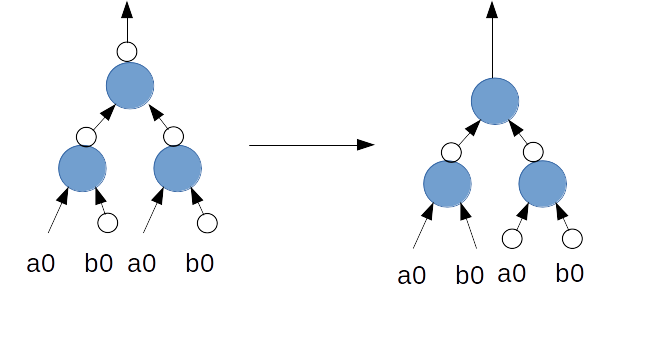
\includegraphics[scale=.5]{Graph.png}
\caption{XOR replacement.}
\label{fig:Diagram}
\end{center}
\end{figure}
\section{Experimental Results}
The proposed method has been implemented in the Galois Framework\cite{GALOIS} as a Galois application. To test our program, we first use ABC to load a verilog file using the read function and generate a structural hash using the strash function. This restructures the circuit into an AIG, which can then be exported back to verilog using write\_verilog and retain the AIG structure.  We can then invoke our program using gaig filename numthreads to run the AIG rewriting heuristic on the circuit as described in Section 3. \\\indent
Both ABC and our program have built-in timing functions to report the runtime of the algorithm. A few sample runtimes are reported in Table 1.

\begin {table*}[t]
\label{tab:title}
\centering
\begin{tabular}{ |p{2cm}|p{2cm}|p{2cm}|p{2cm}|p{2cm}|p{2cm}|p{1cm}|p{1cm}| }
\hline
\multicolumn{6}{|c|}{Algorithm runtimes (averaged over 10 iterations)} & \multicolumn{2}{|c|}{Node Reduction}\\
\hline
Input file & ABC & gaig 1 & gaig 2 & gaig 4 & gaig 8 & ABC & gaig\\
\hline
rca2 & 0.04s & 2.2e-05s & 8.3e-05s & 2.2e-04s & 4.5e-04s & 3 & 3\\
adder16 & 0.03s & 1.5e-04s & 6.4e-04s & 1.75e-03s & 2.99e-03s & 16 & 16\\
mult4 & 0.05 & 8.6e-05s & 4.7e-04s & 8.3e-04s & 1.8e-03s & 17 & 11\\
\hline
\end{tabular}
\caption{Runtimes. rca2 is a simple 2-bit ripple-carry adder, adder16 is a 16-bit adder, and mult4 is a 4-bit multiplier.}
\end{table*}

\section{Conclusion}
Early results are promising, showing that the Galois Framework can be used effectively as a platform to produce a fast, parallelized implementation of the AIG Rewriting heuristic. This is in spite of the fact that our test cases show reduced performance when moving to multiple threads over a single thread, but even then we are still faster than ABC. Such performance reduction is likely a result of the extra overhead incurred by the Galois Framework in determining how to parallelize the graph algorithm execution and in the case of relatively small test cases the extra overhead outweighs the performance improvement of moving to multiple threads. For very large AIGs we would likely see a major performance increase.

\subsection{Further Work}
The first step for anyone wishing to continue this work would be to flesh out the heuristic, adding many more cases beyond XNOR to XOR to cover all common cuts and their substitutions.\\\indent
To improve compatibility of this system with existing AIG software, native support for one of the binary AIG file formats could be implemented. This would also increase the read/write performance of the program with very large AIGs.\\\indent
Another related project that may be valuable would be to implement this same parallelization process for the algorithm on a many-core system (such as a GPU) instead of with the Galois Framework.
\bibliographystyle{acm}
\bibliography{bibfile}

\end{document}

